 In the textbook, language modeling was defined as the task of predicting the next word in a sequence given the previous words. In this assignment, you will implement character-level, word-level N-gram  and character-level RNN language models. You need to both answer the questions and submit your code. You need to submit a zip file to Canvas Homework 3 Programming. This file should contain \texttt{ngram.ipynb}, \texttt{rnn.ipynb} \texttt{hw3\_skeleton\_char.py} and \texttt{hw3\_skeleton\_word.py}. 
 
 You should also submit a zip file to the Gradescope assignment HW3 Language Models. 
 This file should contain \texttt{hw3\_skeleton\_char.py} and \texttt{hw3\_skeleton\_word.py}.

\begin{enumerate}
    \item For N-gram language models, You should complete two scripts \texttt{hw3\_skeleton\_char.py} and \texttt{hw3\_skeleton\_word.py}. Detailed instructions can be found in  \href{https://www.cc.gatech.edu/classes/AY2020/cs7650_spring/hw3/lm/ngram.zip} {\texttt{ngram.ipynb}}. You should also use test cases in \texttt{ngram.ipynb} and use \texttt{ngram.ipynb} to get development results for (c). 
    
    You need to submit a zip file to Gradescope HW3 Language Models. This file should contain \texttt{hw3\_skeleton\_char.py} and \texttt{hw3\_skeleton\_word.py}. You can see the scores for your code there. Character-level N-gram language models accounts for 20 points. Word-level N-gram language models accounts for 10 points, which are bonus for CS 4650. [30pts for CS 7650, 20 pts + bonus 10pts for CS 4650] 

     
    \item See the generation results of your character-level and word-level N-gram language models respectively ($n\geq 1$). The paragraphs which character-level N-gram language models generate all start with \textit{F}. The paragraphs which word-level N-gram language models generate all start with \textit{In}. Did you get such results? Explain what is going on. (CS 4650 can only focus on character-level N-gram language model.) [2 pts]
    
    
    \item (Bonus for CS 4650) Compare the generation results of character-level and word-level N-gram language models. Which do you think is better?  Compare the perplexity of \texttt{nytimes\_article.txt} when using character-level and word-level N-gram language models. Explain what you found. [2pts, bonus for CS 4650]
    
    \item When you compute perplexity, you can play with different sets of hyper-parameters in both character-level and word-level N-gram language models. You can tune $n$ , $k$ and $\lambda$. Please report here the best results and the corresponding hyper-parameters in development sets. For character-level N-gram language models, the development set is \texttt{shakespeare\_sonnets.txt}. For word-level N-gram language models, the development sets are \texttt{shakespeare\_sonnets.txt} and \texttt{val\_e.txt}. (CS 4650 should only focus on character-level N-gram language model.) [6 pts for CS 7650, 2 pts + bonus 4 pts for CS 4650]
    
    \item For RNN language models, You should complete the forward method of Class RNN in  \href{https://www.cc.gatech.edu/classes/AY2020/cs7650_spring/hw3/lm/rnn.zip} {\texttt{rnn.ipynb}}. You need to figure out the code and tune the hyperparameters. You should also copy a paragraph generated by your model and report the perplexity on the development set \texttt{shakespeare\_sonnets.txt}. Compare the results of character-level RNN language model and character-level N-gram language model. [10 pts]

\end{enumerate}


\begin{solution} \ \\
a) Refer to code.	
	
b) The reason ``First'' is always being generated first is because after examining the file shakespeare\_input.txt, you can see the first word is ``First Citizen''. As such, when this entire chunk of text is fed into the model to update the model, the only character that appears after $\sim\sim$ is F. This would actually be cured if we passed several different Shakespeare input files into our model to update it, as each input file (each play) would start with a different word, as such, there would be more variance in the first character generated by the model. In other words, if ``All'' was the first speaker of the play instead of ``First Citizen'', the model would learn to be biased toward starting its text generation with the letter A instead of F.

The reason why ``In'' appears in every instance for the word-level generation is similar. All three word-level models are trained on train\_e.txt, and if you look at the file, it begins with the word ``In''. Furthermore, if you look at the create\_ngram\_model() function, it simply reads in the text from a file without splitting them by lines, so the only instance where ``$\sim$'' appears as the context (with 2 tildas for the 2-gram model, 3 tildas for 3-gram, etc.), is in the case where we see ``$\sim \sim$ In''. As such, the model is biased toward this only occurrence since ``In'' has an insanely high chance of occurring after the tildas.

c) This one is a no brainer: the word-level model is better. The explanation for this is because the character-level model must generate real words, and then once it is successful at generating words that actually exist, it must generate sentences that sound coherent. Meanwhile, the word-level model does not have to worry about the first issue. It already generates real words from a word bank, so the word-level model only has to perform well at stringing those words together into coherent sentences. And this can be seen by the random text generated by both 4-gram character and word-level models. The word-level models do not have any deficiencies in terms of generating realistic words. Their only deficiencies come in terms of generating realistic phrases. 

Now, the quantitative measure, perplexity, was compared between the two interpolation models with the best hyperparameters found in part (d) of this question. For the character-level ngram model, a perplexity of 5.1700 was achieved. Meanwhile, for the word-level ngram model, a perplexity of 1549.9949 was achieved. 

Now, with that being said, it is unfair to compare the word and character level models' perplexities because the shakespeare sonnets test file has a significant number more characters than words, so the probability, or score, is normalized by a larger amount when taking the n-th root. For example, if there were N words, the word-level model would take the N-th root, but if we assume there are 5 letters per word, then there are 5N characters, so the character model would take the (5N)-th root, producing a much smaller score. Additionally, the vocab of the word model is size 62983, and the vocab for the character model is size 67, so there will inherently be different perplexities due to that. One of the reasons this is the case is because when a context does not exist in our model and we assign a uniform probability to a given word or character existing, the word-level model will assign a smaller probability (1/62983) compared to the character level model (1/67).

d) To simplify the process, I first tuned the hyperparameters of the character-level ngram model. First, I tuned the value of $n$, then once I found the optimal $n$, I tuned the value of the lambdas, then I finally tuned the value of $k$. You can see the results (measured through perplexity) below:

$n = 2 \implies 10.2814\\
n = 3 \implies 7.9210\\
n = 4 \implies 6.7296\\
n = 5 \implies 6.1147\\
n = 10 \implies 6.4789$

Then, I took the 5-gram model and tuned the values of the lambdas as follows:

$\left[1, 0, 0, 0, 0, 0\right] \implies 23.4546\\
\left[0, 1, 0, 0, 0, 0\right] \implies 12.5071\\
\left[0, 0, 1, 0, 0, 0\right] \implies 8.1685\\
\left[0, 0, 0, 1, 0, 0\right] \implies 5.9825\\
\left[0, 0, 0, 0, 1, 0\right] \implies 5.5298\\
\left[0, 0, 0, 0, 0, 1\right] \implies 6.2527\\
\left[0.01, 0.01, 0.01, 0.01, 0.9, 0.06\right] \implies 5.2464\\
\left[0.05, 0.05, 0.05, 0.05, 0.75, 0.05\right] \implies 5.2661\\
\left[0.05, 0.05, 0.05, 0.1, 0.5, 0.25\right] \implies 5.1700\\
\left[0.1, 0.1, 0.1, 0.1, 0.4, 0.2\right] \implies 5.4642$

Then, I used lambdas of $\lambda_1 = 0.05, \lambda_2 = 0.05, \lambda_3 = 0.05, \lambda_4 = 0.1, \lambda_5 = 0.5, \lambda_6 = 0.25$ and tuned the values of $k$:

$k = 0.01 \implies 5.1700\\
k = 0.1 \implies 5.4272\\
k = 0.2 \implies 5.6311\\
k = 0.5 \implies 6.0760\\
k = 1.0 \implies 6.6078\\
k = 2.0 \implies 7.3816$

So, as seen above, the best hyperparameters for the character-level model are $n = 5$, lambdas = $\left[0.05, 0.05, 0.05, 0.1, 0.5, 0.25\right]$, $k = 0.01$. For the word-level model, I did the same amount of hyperparameter tuning as I did in the character-level model. So, for the word-level model:

$n = 2 \implies 4649.9847\\
n = 3 \implies 5209.0778\\
n = 4 \implies 5776.3654\\
n = 5 \implies 6315.5207\\
n = 10 \implies 8594.5631$

$\left[1, 0, 0\right] \implies 1549.9949\\
\left[0, 1, 0\right] \implies inf\\
\left[0, 0, 1\right] \implies inf\\
\left[0.9, 0.05, 0.05\right] \implies 1722.2166\\
\left[0.7, 0.15, 0.15\right] \implies 2214.2784\\
\left[0.5, 0.25, 0.25\right] \implies 3099.9898$

$k = 0.01 \implies 1549.9949\\
k = 0.1 \implies 1794.6906\\
k = 0.2 \implies 1897.3396\\
k = 0.5 \implies 2047.2329\\
k = 1.0 \implies 2170.6000\\
k = 2.0 \implies 2313.9570$

So, the best word-level model has $n = 2$, lambdas = $\left[1, 0, 0\right]$, $k = 0.01$. These were validated with the shakespeare\_sonnett.txt set, and after checking perplexity across all parameters on the other dev set, val\_e.txt, the same general patterns hold, so I am certain these parameters are the best ones for the word-level model.

To wrap up, on the same dev set (shakespeare\_sonnett.txt) for the character and word-level models, the perplexity for the character model is 5.1700 and for the word-level model is 1549.9949. For the other word-level dev set, val\_e.txt, I am getting a perplexity of 393.8618 after training on train\_e.txt.

If you want to specifically see these scores, or simulate the same tests, just run ``python3 hw3\_skeleton\_word.py`` and ``python3 hw3\_skeleton\_word.py``. I specifically added the tests in the main() function, so the tests will run immediately after calling the program.

Below are two screenshots. The first one shows the perplexity outputs from the character-level model in the order I presented above. The second screenshot shows the perplexities output from the word-level model in the order I presented above. Both were the output after training on shakespeare\_input.txt and testing on shakespeare\_sonnets.txt. I did not show results on val\_e.txt for brevity's sake.

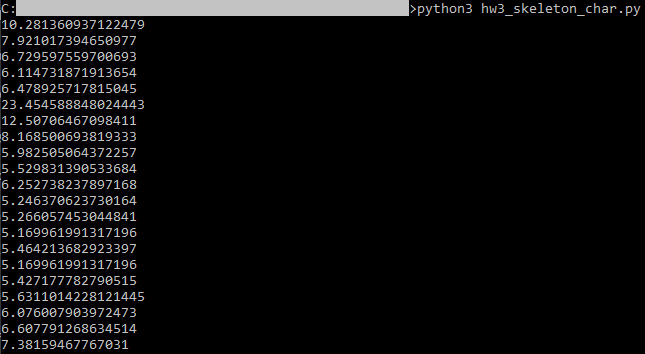
\includegraphics[scale=0.9]{4d-character-model}

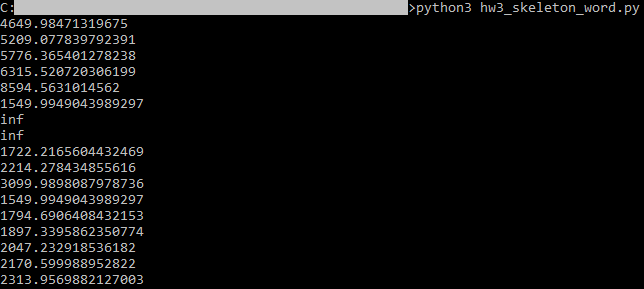
\includegraphics[scale=0.9]{4d-word-model}

e) After evaluating on ``shakespeare\_sonnets.txt'', I obtained a perplexity of 6.8739 on the character-level RNN. One sample from the character-level RNN with temperature of 0.2 is the following:\\

``The hath he speak he come.

SARDONA:
I have he be the best the grown and he be be and for the speak.

PERDARIUS:
What hath the come the come the come and hath the come.

CROSANDO:
I have the come the pr''\\

Please ignore the quotations. I added those purely as an indicator it is output from the model, rather than something I directly typed. Now, we can compare this to a sample paragraph from the character-level 4-gram language model:\\

``"First Apollows-monstands. The foundly and highness' friend.\textbackslash n\textbackslash nCOSTARD:\textbackslash nThe would first Guard:\textbackslash nJoin while he days I true:\textbackslash nI have the reputation, good:\textbackslash nBut a tradian a prithers.\textbackslash n\textbackslash nTOUCHSTONE:\textbackslash nSoft,\textbackslash nthough they lief talend mud indeed, double your treason "''\\

Once again, the pair of quotations inserted at the beginning and end of the paragraph were inserted by me, but all the other quotations were generated by the model. In general, both models perform terribly in terms of generating coherent text that is easily readable by English speakers. However, I will say the 4-gram model performed slightly better in terms of coherency, although marginal. The RNN generated sequences such as ``the come the come the come and hath the come'' which makes no sense at all, while the 4-gram model generated phrases such as ``I have the reputation, good'', which is significantly easier to read and comprehend. Meanwhile, the RNN generated more realistic paragraphs in the sense that the RNN-generated text looks like it just came out of a playbook, because it is well-structured (i.e. a character, ``SARDONA'', is specifically speaking at a certain time). Now, with that being said, I will not paste the paragraphs for the 3-gram or 2-gram ngram character models, but those are significantly worse than the character RNN. As such, I will say the 4-gram character model works better than the RNN character model, in terms of qualitative analysis, but the RNN character model performs leaps and bounds better than the 2-gram and 3-gram models in terms of generating coherent paragraphs, text, and words.

With that being said, when comparing the two models quantitatively, namely through perplexity, the ngram model performs better. Through the character-level ngram model, the perplexity is 5.1700 (as mentioned in question 4d). Meanwhile, the RNN generated a sentence with perplexity of 6.8739, which is worse than the ngram model. As such, I believe the ngram model does a better job at selecting words, under uncertainty, that actually have a chance of appearing. Therefore, since I believe the 4-gram ngram model does a better job qualitatively, and it has shown to perform better quantitatively, the 4-gram model is better than the RNN.
\end{solution}